\chapter{Implementation}
The \textit{Confuzzer} system was implemented with a combination of the Intel
PIN tool to do binary instrumentation and Taint Analysis, and the z3 Python
bindings to actually perform the Concolic Execution step. The current version of
the system is available online at \url{https://github.com/dvorak42/confuzzer}.
The rest of this chapter will discuss the implementation of each of these parts,
as well as the distributed and graphing components.

\section{PIN Taint Analysis Tool}
In order to do the Taint Analysis on the binary, we ended up implementing an
extension for PIN, an Dynamic Binary Instrumenter, to keep track of the tainted
state of memory and registers, and to build up a list of all the instructions
that operated on tainted locations. 

Instead of using a full-system emulator, we ended up choosing to use
an application-specific Dynamic Binary Instrumenter (DBI), since it should have
a lower overhead than emulating an entire system. Of the popular choices, we
ended up using PIN since it was one of the few DBI tools that worked without any
need for compile-time injection and allowed us to fully instrument the program
with easy access to the state of the registers and memory throughout the
program \cite{pintool}. Another option was DynamoRIO, another similar DBI,
however there were fewer systems built on top of it, and had less support at the
time.

The PIN plugin takes in the binary that is being analyzed, as well as the names
of the tainted inputs to the binary. In order to keep track of tainted values,
we first use PIN to instrument any syscalls. Before each syscall, we check the
type of the syscall and if it is an ``open'', we check whether the argument is
one of the tainted files that was passed in, and if so keep track of the file
descriptors referencing these tainted files. Once we have an open tainted file,
we need to check for ``read'' syscalls and label and taint any memory that is
written by the ``read'' syscall.

Once we have a tainted memory location, we need to start instrumenting all
instructions to check whether they are reads from either tainted memory or
registers. Since we need to parse the actual registers and memory locations that
are being affected by the we have different instrumentation functions based on
the number of operands for each operation, and whether they affect registers or
memory locations.

The one special case we need to deal with separately is adding an additional
``branch'' point before predicated instructions. This way, every time that the
predicated instruction, we create a new branch point dependent on the state of
the RFLAG register. The one problem with this approach is that every instruction
will end up instrumented, since we also need to keep track when the taint on
registers and addresses are cleared.

In order to keep track of registers and addresses, we create separate lists for
each. However, since we have instructions that move different size operands, for
each register, we need to separately keep track of each chunk in a
register. While we can do bit-level chunking, x86 primarily affects registers at
a byte level, so the current implementation uses byte-sized chunks. We also
normalize all registers to the largest size ($RDI, RSI, RAX, RBX, \ldots$) when
keeping track of the registers. We also need to keep track of the ID of each
register, so that as we parse new operations that modify the value of the
register, we store it in a newly named variable.

\begin{figure}[ht]
 \centering
\begin{verbatim}
taintRegToReg(instruction, srcReg, dstReg):
  chunkStart, chunkEnd = instruction.offset, instruction.size
  affectReg = []
  for(i in sizeof(dstReg)):
    r1 = {dstReg, i, dstReg.id}
    r2 = {dstReg, i, dstReg.id+1}
    if i < instruction.offset or i > instruction.size + instruction.offset:
      taintEquations.append({'=', r1, r2})

  if isTainted(srcReg):
    s1s = srcReg[chunkStart:chunkEnd]
    s1c = {srcReg, chunkEnd-chunkStart}
    d1s = dstReg[chunkStart:chunkEnd]
    d1c = {dstReg, chunkEnd-chunkStart}
    taintEquations.append({'=', s1s, s1c})
    taintEquations.append({instruction, s1c, d1c})
    taintEquations.append({'=', d1c, d1s})
  else:
    for(i in [chunkStart, chunkEnd]):
      removeTaint(dst)
\end{verbatim}
 \caption{Taint Spread Pseudo-code}
 \label{figure:taintcode}
\end{figure}


Figure \ref{figure:taintcode} shows the pseudocode for actually spreading taint
around the various registers and addresses the program accesses. For any
operations that use tainted registers and addresses, we increment the ID of the
registers being written and then taint them, as well as adding a constraint
representing the assembly instruction. Since we don't want to create constraints
for all registers, we also need to get the value of operands that aren't
tainted. We do this by copying the memory from the source operand, or by using
the Register context that we have to get the current value of an address.

We also need to clear the tainted flag on register and addresses whenever we
have an instruction that moves non-tainted values into a register. Without
clearing the taint flags, we would end up with almost all the registers and
addresses accessed by the program after the original tainted file is read.

Finally we need to keep on propagating any parts of the register that weren't
affected by the current instruction. This is actually a simplification of the
actual code since we need to cast the register chunks together so that the
instruction can operate on them, and then cast it back into separate chunks for
further instructions to interact with.

Whenever we encounter a branching point in the program execution, we check
whether the RFLAGS register is currently tainted, and if so we add the branch to
the list of tainted branches, along with the current value of the RFLAGS
register. This allows us to keep track of which direction each branch was taken
in. While we could keep track of this by checking what the next executed
instruction is, that would require extra bookkeeping.

Separate from the Taint Analysis, we also instrument exception handling in order
to deal with the case of segfaults and other crashes. Since we can't trust that
standard file descriptors for user input and output are still available at this
point, we have to wait until the end of the program's execution to record the
crash/segfault.

At the end of the program's execution, we store all the branching points and
taint constraints in a file for the Concolic Execution System to parse and use
to determine new constraints. In addition, if we recorded a crash or overflow
issue, we also update the execution log with that data. Once we've finished with
the current execution, the Concolic System then takes over to generate new test
cases.

\section{Concolic System}
The Concolic System is implemented using a combination of Python and z3 bindings
to parse the file received from the Taint Analysis system. Every time we receive
the analysis, we parse it in two stages. The first stage parses the taint
constraints into formulas, and the second stage creates the z3 equations.

The first stage parses out the opcode from the assembly instruction and turns it
into symbolic notation. We have to do the parsing in two stages since we need to
build up the set of variables that will be used by the SMT solver. Some of the
assembly opcodes don't have a direct translation to a symbolic equation since we
have a limited set of operations we can use with the SMT solver.

The second stage is where we actually create the z3 variables and the
constraints are actually added to the system. We mark the z3 variables
representing the tainted file inputs differently so that we can later build up
the new input file.

We also have a third stage for our actual branch conditions where we use the
branch opcode and the value of the RFLAGS register at that time to figure out
whether we actually took the TRUE or FALSE path.

Once we've finished parsing all the branches and taint constraints, we can start
iterating through each of them and building up a new path constraint using the
branches we select for this loop and the rest of the taint constraints. Since we
don't have any circular dependencies, and most of the constraints are fairly
straightforward, z3 works fairly well at solving the constraints for satisfiable
sets of constraints, while converging to unsatisfiability for the paths that are
unreachable.

In order to maximize the parts of the program we are exploring early on, we
iterate through each branch on the path and keep the previous branch directions,
while flipping the direction we are exploring on the current branch. So we
create $N$ new paths for every path with $N$ branching points. We then
de-duplicate the repeated paths/inputs once we've converted the solutions from
the SMT solver into actual input files. A good number of paths will end up being
unsatisfiable since there are no inputs to reach that path, or there are
contradictory branches from non-optimized or dead code.

Once we've solved the constraint equations, we generate a new test input and
place it into a test input queue. Its during this phase that we check whether
the input and paths match any of our prioritized branches and if so, we increase
their priorities in the Taint Analysis stage. We keep on parsing outputs and
generating new paths until we work through our queue of inputs and are unable to
generate new unique paths. We also keep track of any paths which result in
crashes/segfaults and mark those as interesting inputs.

\section{Additional Components}
While the previous parts are sufficient to actually run the fuzzer, there are
a few additional components to improve the system. We also have implemented a
distributed system and graph visualization to help with the usability and
efficiency of the system.

We use xmlrpclib and synchronized Queues in order to communicate between the
master and each of the workers. The system is designed to allow each server to
support multiple workers per machine. Each worker can run in separate threads,
listening for the master using different ports. Additionally, each worker thread
can run multiple PIN Taint Analysis processes simultaneously. This allows us to
run about 64 analysis operations at the same time, with 8 threads per machines
on 8 servers.

To prevent security issues with the RPCs being maliciously used, we require that
the binaries that are being used are uploaded to each server through a separate
channel. We also have a script that separately fetches all the log files from
each run through of the taint analysis in order to store any additional
information that the user might want to look over for the crashing test cases.

\begin{figure}[t]
 \centering
 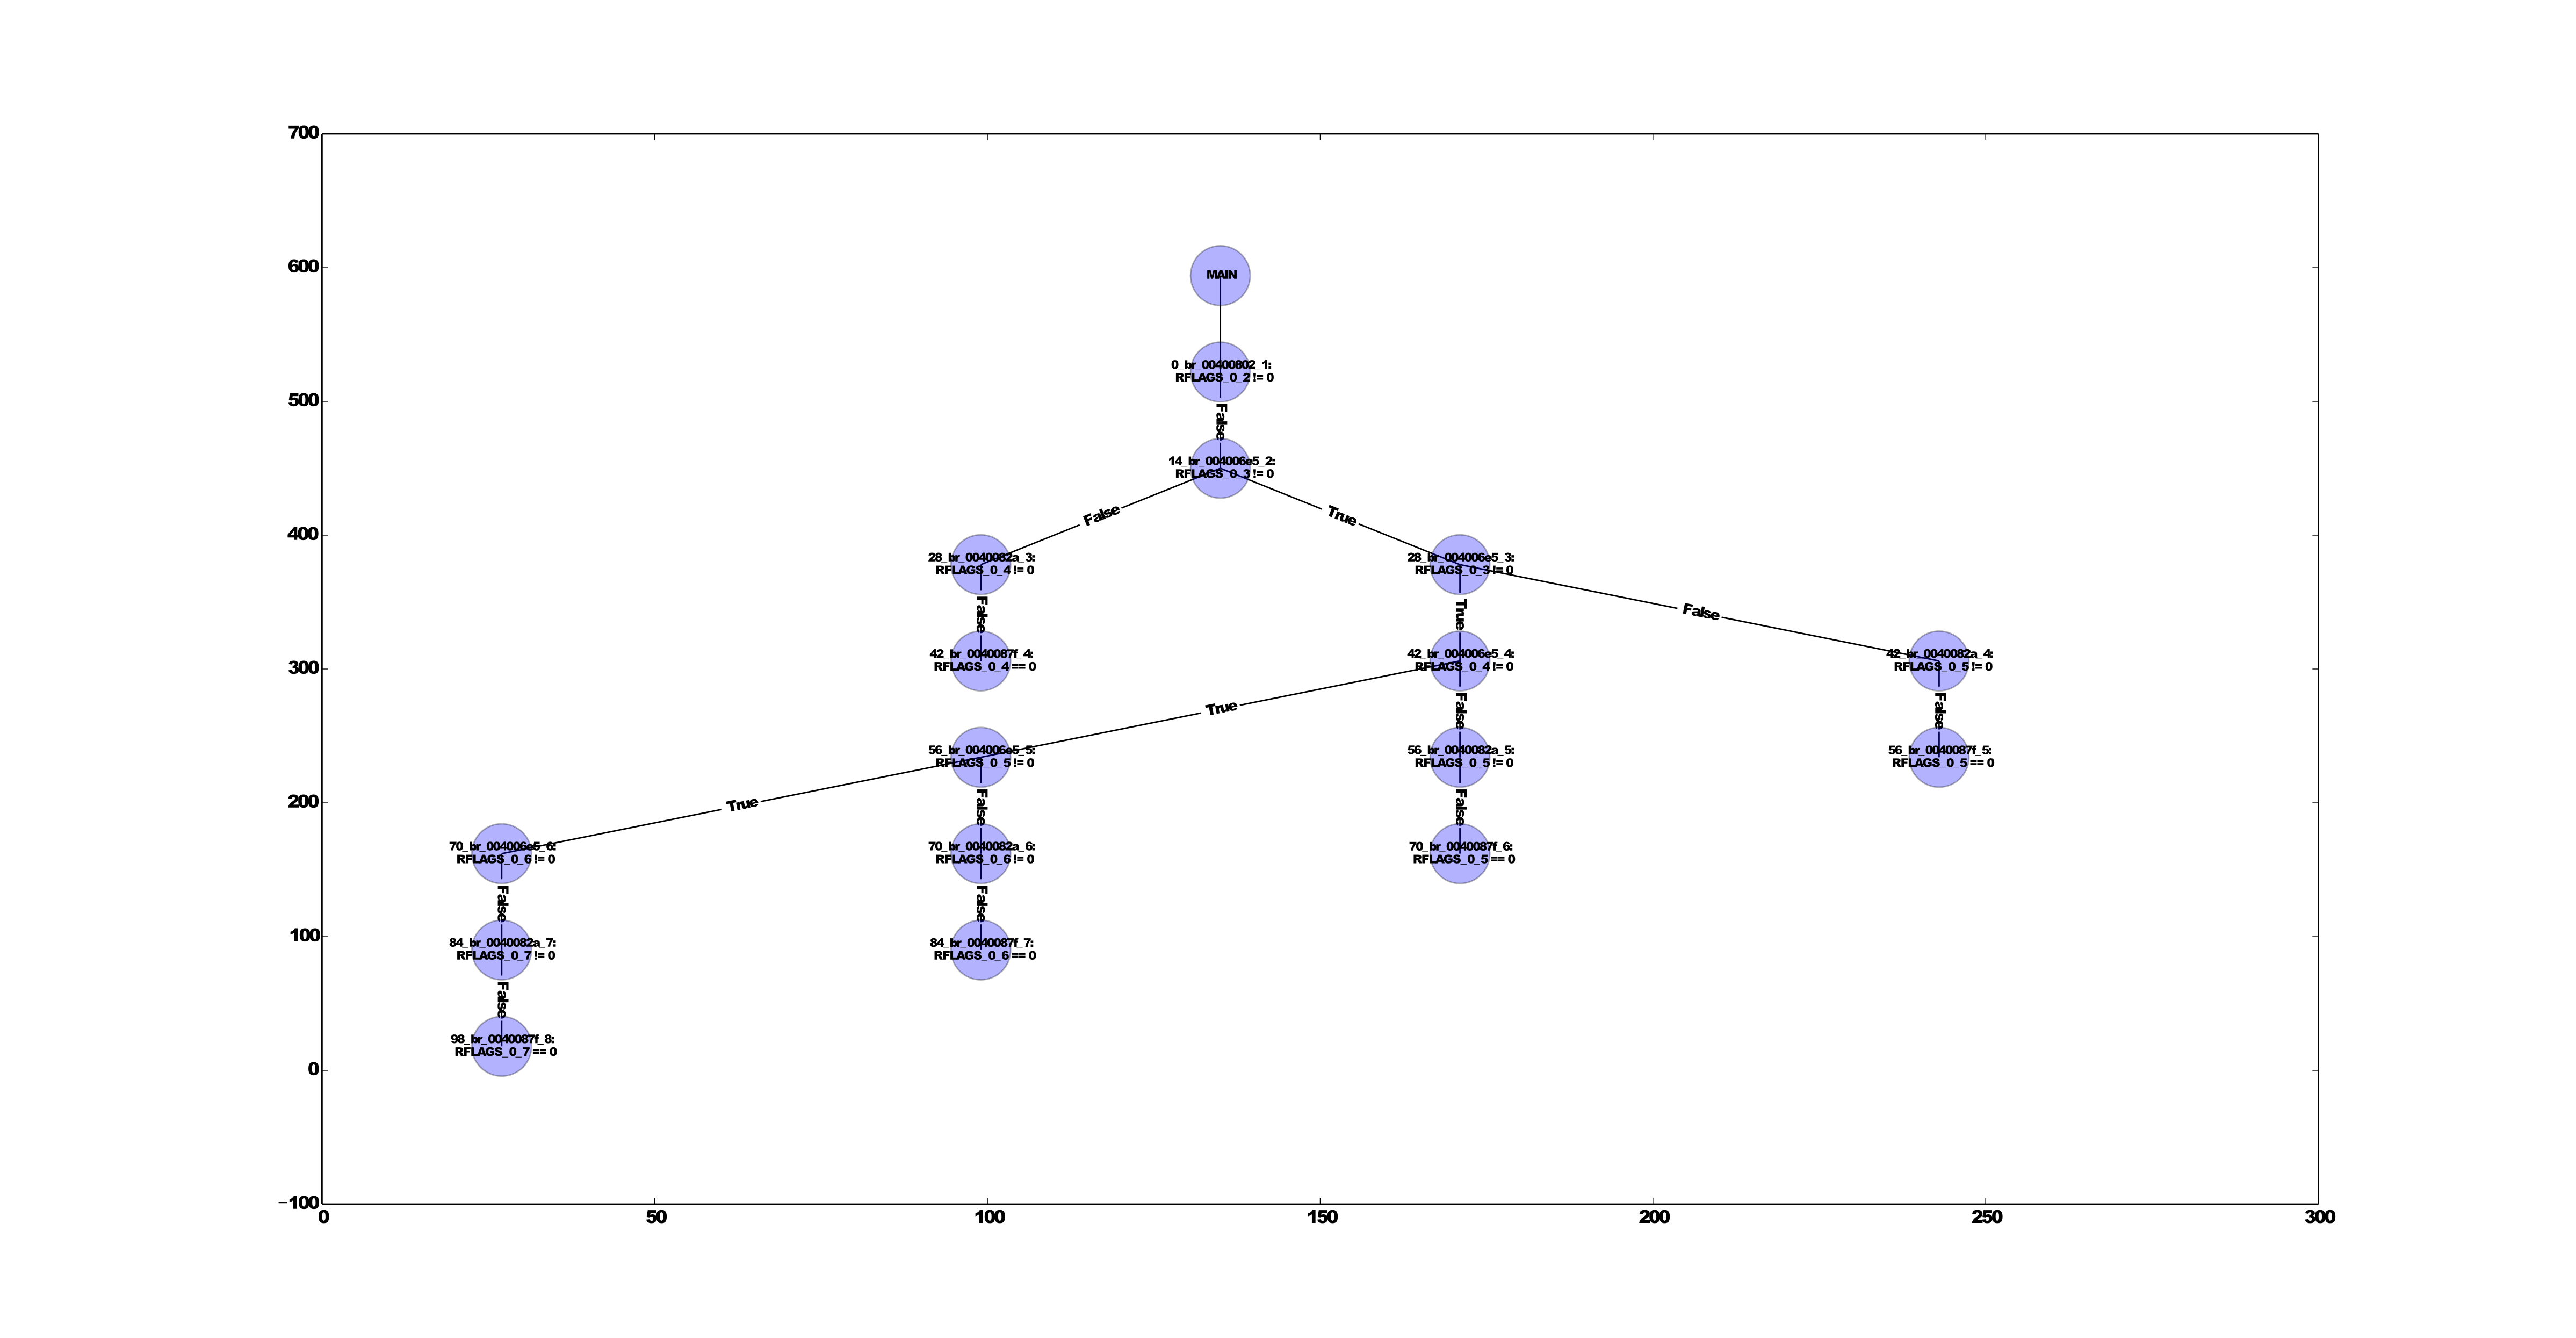
\includegraphics[width=\textwidth]{graphs/1_7}
 \caption{Example Execution Graph}
 \label{figure:samplegraph}
\end{figure}

We use pyplot and graphviz to actually generate the graph of the program
execution. Figure \ref{figure:samplegraph} shows the graph that is generated as
part of the execution of binary. In order to give the user an idea of which
branch each node represents, we also include the assembly instruction that
actually represents the branch.

The user can then input the name of a branch from the graph image into the main
thread in order to prioritize it. Since each node is uniquely identified,
the name of the branch also includes the prefix branches. The user can
prioritize multiple branches in the same part of the program in order to have
the system focus on a specific section of the binary.

While these components don't change the correctness of the system, it does make
the system faster and allow for the user to prioritize parts of the program that
they believe to be vulnerable or critical. There are some additional
optimizations that could be made that will be mentioned in the \textbf{Future
  Work} section in Chapter 6.